\documentclass{beamer}

\graphicspath{{./images/}}

\usetheme{Berlin}
\title{{\tt OOPS}: An $S5_n$ Prover for Educational Settings}
\author{Gert van Valkenhoef \and Elske van der Vaart \and Rineke Verbrugge}
\date{12 October, 2009}

\logo{
\includegraphics[height=0.5cm]{RUGR_logoEN_rood_RGB}}

\begin{document}

\begin{frame}
\maketitle
\end{frame}

\section{Introduction}
\subsection{}

\begin{frame}
\frametitle{What is {\tt OOPS}?}
\begin{itemize}
\item {\tt OOPS}: Object Oriented Prover for $S5_n$
\item Proven Sound \& Complete, Correct
\item Implemented in Java:
	\begin{itemize}
	\item cross-platform
	\item widely understood
	\item long-lived
	\end{itemize}
\item Click \& Run
\item Open Source (GPL):
	\begin{itemize}
	\item Get the source: http://github.com/gertvv/oops
	\end{itemize}
\item Aimed at students learning $S5_n$
\end{itemize}
\end{frame}

\begin{frame}
\frametitle{Why {\tt OOPS}?}
\begin{itemize}
\item Started as a Multi-Agent Systems (MAS) student project
\item Out of frustration with the LWB
	\begin{itemize}
	\item Binary blob with archaic dependencies
	\item Hard to get working
	\item No $S5_n$ support
	\end{itemize}
\item Because we want those with frustrations about {\tt OOPS} to have the power to do something about it!
\end{itemize}
\end{frame}

\begin{frame}
\frametitle{What {\tt OOPS} is {\em not}}
\begin{itemize}
\item Our proof method is not:
	\begin{itemize}
	\item Highly innovative
	\item Super efficient
	\item Very complicated
	\end{itemize}
\item A competitor to the Tableaux Workbench
	\begin{itemize}
	\item Our aim is not to support research in new logics
	\end{itemize}
\end{itemize}
\end{frame}

\section{The Prover}
\subsection{}

\begin{frame}
\frametitle{The Prover}
\begin{itemize}
\item Implementation of {\bf ELtap} (by Matthijs de Boer)
\item Uses labeled tableaux
\item Was proven (by me) to be Sound \& Complete
\item Complexity class: {\sc expspace}
	\begin{itemize}
	\item Problem for large theories
	\item Algorithm is easy to replace (little coupling)
	\end{itemize}
\item Details in the paper (and references)
\end{itemize}
\end{frame}

\begin{frame}
\frametitle{Features (overview)}
\begin{itemize}
\item One-click run (no installation)
\item Visualize tableaux
\item Generate / visualize counter-models
\item Integrated scripting (Lua)
	\begin{itemize}
	\item Build agents that use {\tt OOPS} to reason
	\end{itemize}
\item Basic graphical user interface
\end{itemize}
\end{frame}

\section{Demo}
\subsection{}

\begin{frame}
\frametitle{Demonstration}
\begin{itemize}
\item Hopefully, I can do a live demonstration
\item ... and skip the next few slides
\end{itemize}
\end{frame}

\begin{frame}
\frametitle{Demonstration}
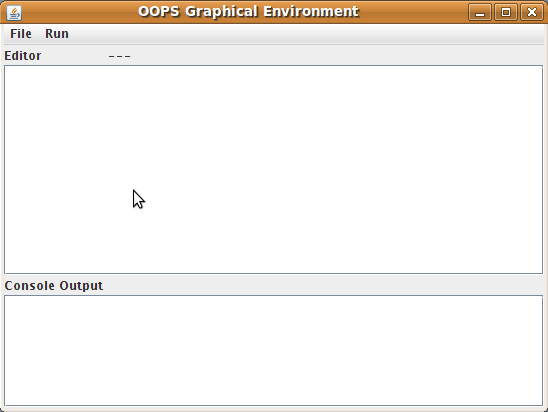
\includegraphics[width=0.7\textwidth]{demo01}
\end{frame}

\begin{frame}
\frametitle{Demonstration}
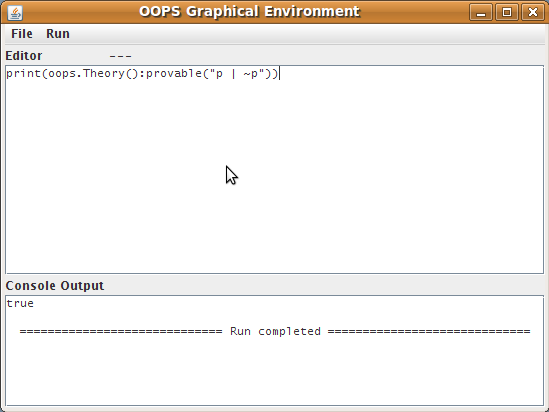
\includegraphics[width=0.7\textwidth]{demo02}
\end{frame}

\begin{frame}
\frametitle{Demonstration}
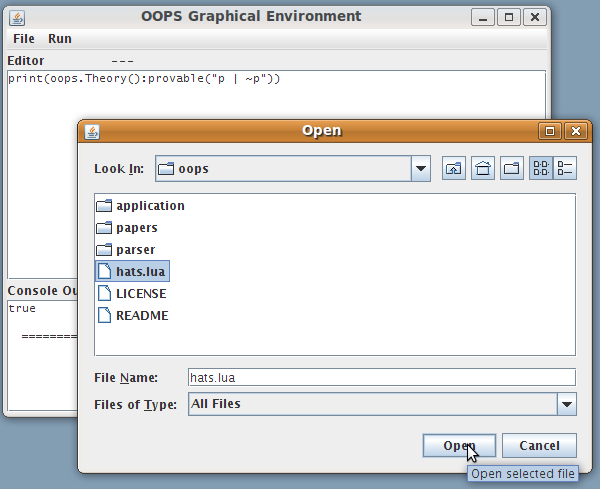
\includegraphics[width=0.8\textwidth]{demo03}
\end{frame}

\section{Conclusion}
\subsection{}

\begin{frame}
\frametitle{Conclusion}

\end{frame}

\begin{frame}
\frametitle{Future Work}

\end{frame}

\end{document}
